% Local Customization
% !TEX root = ../../Build/main.tex
% 
% Copyright Statement
% ###################################################################
% Copyright (c) 2018, Marc De Graef 
%  Editors: A.D. Rollett & M. De Graef
% All rights reserved.
%
% Licensed under the Creative Commons CC BY-NC-SA 4.0 License, 
% hereafter referred to as the "License"; you may not use this 
% document except in compliance with the License. You may obtain 
% a copy of the License at 
%     https://creativecommons.org/licenses/by-nc-sa/4.0/legalcode 
% Unless required by applicable law or agreed to in writing, all 
% material distributed under the License is distributed on an 
% "AS IS" BASIS, WITHOUT WARRANTIES OR CONDITIONS OF ANY KIND, 
% either express or implied. See the License for the specific 
% language governing permissions and limitations under the License.
% ###################################################################
%
% Chapter Parameters
% ###################################################################
%\corechapter{Yes}   % uncomment this line only if this chapter is a core/foundational chapter;
\OCchapterauthor{Marc De Graef, Carnegie Mellon University} %this will appear in a secondary header below the chapter title.

% graphics path for all figure *.eps files 
\renewcommand{\chaptergraphicspath}{src/Crystallography/eps/}

%	redefine the \chabbr command to be a six-character string that uniquely identifies this 
%	chapter; easiest way to do this is to take the first couple of letters from the title words
\renewcommand{\chabbr}{BASCRY}

%     replace \noheaderimage by the chapter header image file name (without .eps extension).
%     Chapter header images must be 2480 x 1240 pixels with 300dpi, RGB format.
\chapterimage{\noheaderimage}

%	Make sure to use the \OClabel{} command everywhere instead of \label{} !
\chapter{Basic Crystallography}\OClabel{Crystallography}

% add the author information so that it will appear in the Author List at the start of the document
\writeauthor{BASCRY:Crystallography}{Basic Crystallography}{De Graef}{Marc}{Materials Science and Engineering}{Carnegie Mellon University}{mdg@andrew.cmu.edu}{https://www.mse.engineering.cmu.edu/directory/bios/degraef-marc.html}

% Each chapter begins with Learning Objectives; the list of objectives should have links to sections/subsections using their OC labels
% each Learning Objective should be an active statement (i.e., contain a verb).  The \\ command can be used to force an item into the 
% second column if LaTeX breaks the line at an awkward location.
\lightgraybox{\begin{center}
    {\LARGE\sffamily\bfseries {\color{OCBurntOrange}\textbf{Learning Objectives}}}\\[1em]
\end{center}

{\color{OCalmostblack}\sffamily
\begin{multicols}{2}
\begin{itemize}
    \item[{\color{OCBurntOrange}\OCref{nonCartesian}:}] Learn how to work with vectors in a non-Cartesian reference frame
    \item[{\color{OCBurntOrange}\OCref{worldviews}:}] Learn about two world views
    \item[{\color{OCBurntOrange}\OCref{lattices}:}] Enumerate crystal systems and Bravais lattices
    \item[{\color{OCBurntOrange}\OCref{crystalcomputations}:}] Perform non-Cartesian computations
    \item[{\color{OCBurntOrange}\OCref{transform}:}] Transform between direct and reciprocal space
    \item[{\color{OCBurntOrange}\OCref{Cartesian}:}] Connect back to the good old Cartesian reference frame    
    \item[{\color{OCBurntOrange}\OCref{usefulcomp}:}] Learn about other useful crystallographic computations
\end{itemize}
\end{multicols}}}
% ###################################################################
% ###################################################################
% ###################################################################



\section{Vectors in Non-Cartesian Reference Frames}\OClabel{nonCartesian}

\subsection{Basic vector operations\OClabel{ssec:vectoroperations}}
We will represent vectors by bold symbols, e.g.,  $\mathbf{a}$, $\mathbf{b}$, $\ldots$.  Unless stated otherwise, we will work with Cartesian (i.e., orthonormal) reference frames\index{Cartesian reference frame}; Cartesian basis vectors\index{Cartesian basis vector} will always be represented by vectors of the type $\mathbf{e}_i$, where the subscript $i$ can take on the values $1, 2, \ldots, D$ and $D$ is the dimension of the space in which the vectors live.  Occasionally, the subscript $i$ will be interpreted to mean $x, y$ in 2D and $x,y,z$ in 3D; this will be clear from the context, and usually this notation is only used to clarify things.  Note that vectors represented by the letter ``\textbf{e}'' will always be assumed to be unit vectors.\index{unit vector}

\begin{wrapfigure}{r}{0.3\textwidth}
  \centering\leavevmode
\Ovalbox{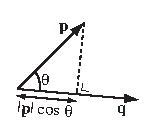
\includegraphics[width=0.28\textwidth]{dotproduct}}
\caption{\small Illustration of the vector dot product as the projection of $\mathbf{p}$ onto $\mathbf{q}$, multiplied by the length $\vert\mathbf{q}\vert$.}
\OClabel{fig:dp}
\end{wrapfigure}

The dot product\index{dot product} between two vectors (see Fig.~\OCref{fig:dp}) is denoted by the symbol $\cdot$, as in:
\begin{equation}
	\mathbf{p}\cdot\mathbf{q} = \vert\mathbf{p}\vert\vert\mathbf{q}\vert\cos\theta \ ,\OClabel{eq:dotproduct}
\end{equation}
where $\vert\mathbf{p}\vert$ stands for the norm (length) of the vector $\mathbf{p}$, and $\theta$ is the angle between the two vectors. When two vectors are perpendicular to each other, then their dot product vanishes.  The dot product of a vector with itself results in the square of the length of the vector, or
\begin{equation}
	\vert\mathbf{p}\vert = \sqrt{\mathbf{p}\cdot\mathbf{p}} \ .\OClabel{eq:vectorlength}
\end{equation}

The vector cross product\index{vector cross product}\index{cross product} is represented by the symbol $\times$, as in
\begin{equation}
	\mathbf{p}\times\mathbf{q} = \vert\mathbf{p}\vert\vert\mathbf{q}\vert \sin\theta\ \mathbf{e}^{\perp} \ ,\OClabel{eq:crossproduct}
\end{equation}
Here, the unit vector $\mathbf{e}^{\perp}$ is perpendicular to both $\mathbf{p}$ and $\mathbf{q}$, such that $\mathbf{p}$, $\mathbf{q}$ and $\mathbf{e}^{\perp}$ form a right-handed reference frame.\footnote{In crystallography and texture analysis we always use right-handed reference frames. Left-handed frames are common in computer vision and animation.}   The cross product of a vector with itself always vanishes. The mixed vector product,\index{mixed vector product} $\mathbf{p}\cdot(\mathbf{q}\times\mathbf{r})$, is equal to the volume, $V$, of the parallellepiped generated by the three vectors.  For a right-handed reference frame, the mixed vector product is always positive; for  a left-handed reference frame it is negative.

Vector components are represented by subscripted italic symbols; the Cartesian components of the vector $\mathbf{p}$ can be determined by projecting the vector onto each coordinate axis using the dot product.  Thus, we have:
\begin{equation}
	\mathbf{p} = \sum_{i=1}^{D}(\mathbf{p}\cdot\mathbf{e}_i)\mathbf{e}_i = \sum_{i=1}^D p_i\mathbf{e}_i \ .
\end{equation}
We will use the Einstein summation convention:\index{summation convention} \textit{when a subscript is present twice on the right hand side of an equation, a summation over that subscript is implied and the summation sign need not be written}.  
Thus, we have:
\begin{equation}
	\mathbf{p} = p_i\mathbf{e}_i\quad\text{with}\quad p_i = \mathbf{p}\cdot\mathbf{e}_i \ .
\end{equation}

\noindent In component notation, the vector dot and cross products can be written explicitly as follows:
\begin{itemize}
	\item For the dot product between $\mathbf{p}$ and $\mathbf{q}$ we have:
	\[
		\mathbf{p}\cdot\mathbf{q} = (p_i\mathbf{e}_i)\cdot(q_j\mathbf{e}_j)
		= p_i (\mathbf{e}_i\cdot\mathbf{e}_j) q_j \ .
	\]
	The dot product of the orthonormal basis vectors is equal to $1$ for $i=j$ or $0$ for $i\ne j$; we represent this by the Kronecker symbol\index{Kronecker symbol} $\delta_{ij}$, which corresponds to the $D$-dimensional identity matrix:
	\[
		\mathbf{p}\cdot\mathbf{q} = p_i \delta_{ij} q_j \ .
	\]
	Carrying out the summation over $j$ we obtain:
	\[
		\mathbf{p}\cdot\mathbf{q} = p_i q_i \quad [=p_1q_1+p_2q_2+\ldots ]\ .
	\]
	Using $x,y,\ldots$ as the subscripts, we obtain the familiar expression $\mathbf{p}\cdot\mathbf{q} =p_xq_x+p_yq_y+\ldots$.
	\item For the vector cross product we have:
	\[
		\mathbf{p}\times\mathbf{q} = p_iq_j \epsilon_{ijk} \mathbf{e}_k \ ,
	\]
	where $\epsilon_{ijk}$ is the permutation symbol\index{permutation symbol}; this symbol is equal to $+1$ if $ijk$ is an even permutation of $123$, $-1$ for an odd permutation, and $0$ whenever two or more of the indices are equal.  This definition leads to the familiar expression:
	\[
		\mathbf{p}\times\mathbf{q} = (p_2q_3-p_3q_2)\mathbf{e}_1 +(p_3q_1-p_1q_3)\mathbf{e}_2 +(p_1q_2-p_2q_1)\mathbf{e}_3 \ .
	\] 
\end{itemize}

\subsection{Transformation of a vector}\OClabel{vectortransformation}
Let us consider two Cartesian reference frames, one given by the 
orthonormal triplet $\{\mathbf{e}_x,\mathbf{e}_y,\mathbf{e}_z\}$, the second by 
the triplet 
$\{\mathbf{e}_x^{\,\prime},\mathbf{e}_y^{\,\prime},\mathbf{e}_z^{\,\prime}\}$.  
We also consider a vector, $\mathbf{q}$; this vector has components $q_j$ with respect 
to the reference frame $\mathbf{e}_j$, so that $\mathbf{q}=q_j\mathbf{e}_j$.  
The vector $\mathbf{q}$ also has components $q'_i$ with respect to the vectors $\mathbf{e}'_i$.  
We begin by writing the vector $\mathbf{q}$ as:
\[
	\mathbf{q} = q_j\mathbf{e}_j\qquad (= q_x\mathbf{e}_x + q_y\mathbf{e}_y+q_z\mathbf{e}_z).
\]
When we take the dot product with $\mathbf{e}_x$, we obtain:
\[
	\mathbf{q}\cdot\mathbf{e}_x = q_j \mathbf{e}_j\cdot\mathbf{e}_x;
\]
since the basis vectors are orthonormal, we have
\[
	\mathbf{q}\cdot\mathbf{e}_x = q_j \delta_{jx} = q_x.
\]
Hence, the component $q_x$ is determined by projecting the vector $\mathbf{q}$ onto the 
basis vector $\mathbf{e}_x$.  The same is true for the other components:
\[
		q_y = \mathbf{q}\cdot\mathbf{e}_y;\qquad
		q_z = \mathbf{q}\cdot\mathbf{e}_z.
\]
Therefore, we can write the vector $\mathbf{q}$ as:
\[
	\mathbf{q} = (\mathbf{q}\cdot\mathbf{e}_j) \mathbf{e}_j.
\]
This must be valid for every vector $\mathbf{q}$, so in particular it must be valid for $\mathbf{q}=\mathbf{e}'_x$:
\[
	\mathbf{e}'_x = (\mathbf{e}'_x\cdot\mathbf{e}_j) \mathbf{e}_j.
\]
A similar relation results for $\mathbf{e}'_y$ and $\mathbf{e}'_z$:
\[
	\mathbf{e}'_y = (\mathbf{e}'_y\cdot\mathbf{e}_j) \mathbf{e}_j\qquad \mathbf{e}'_z = (\mathbf{e}'_z\cdot\mathbf{e}_j) \mathbf{e}_j.
\]
In general, we write
\[
	\mathbf{e}'_i = (\mathbf{e}'_i\cdot\mathbf{e}_j) \mathbf{e}_j;
\]
Then we introduce the transformation matrix $\alpha_{ij}$, defined as:
\[	
	\alpha_{ij} \equiv \mathbf{e}'_i\cdot\mathbf{e}_j.
\]
Explicitly, the transformation matrix is given by:
\[
	\alpha_{ij} = \left(\begin{array}{ccc}
	\mathbf{e}'_x\cdot\mathbf{e}_x & \mathbf{e}'_x\cdot\mathbf{e}_y & \mathbf{e}'_x\cdot\mathbf{e}_z\\
	\mathbf{e}'_y\cdot\mathbf{e}_x & \mathbf{e}'_y\cdot\mathbf{e}_y & \mathbf{e}'_y\cdot\mathbf{e}_z\\
	\mathbf{e}'_z\cdot\mathbf{e}_x & \mathbf{e}'_z\cdot\mathbf{e}_y & \mathbf{e}'_z\cdot\mathbf{e}_z\end{array}\right)=
	\left(\begin{tabular}{ccc}\centering $\alpha_{xx}$ & 
$\alpha_{xy}$ & $\alpha_{xz}$ \\
$\alpha_{yx}$ & $\alpha_{yy}$ & $\alpha_{yz}$ \\
$\alpha_{zx}$ & $\alpha_{zy}$ & $\alpha_{zz}$ \\
\end{tabular}\right)
\]
In general, the relation between the two sets of basis vectors can be 
written as~:
\begin{eqnarray}
\mathbf{e}_x^{\,\prime}&=&\alpha_{xx}\mathbf{e}_x+\alpha_{xy}\mathbf{e}_y+\alpha_{xz}\mathbf{e}_z\nonumber\\
\mathbf{e}_y^{\,\prime}&=&\alpha_{yx}\mathbf{e}_x+\alpha_{yy}\mathbf{e}_y+\alpha_{yz}\mathbf{e}_z\\
\mathbf{e}_z^{\,\prime}&=&\alpha_{zx}\mathbf{e}_x+\alpha_{zy}\mathbf{e}_y+\alpha_{zz}\mathbf{e}_z\nonumber
\end{eqnarray}
or, in index notation:
\begin{equation}
	\mathbf{e}'_i = \alpha_{ij}\mathbf{e}_j.\OClabel{eq:alphadef}
\end{equation}
This is a \textit{linear} relation, known as a \textit{coordinate 
transformation}.\index{coordinate transformation}  We will assume throughout this text that the 
origin itself does not change during the coordinate transformation.  
If there were a change in the position of the origin as well, then we 
would have to add a translation vector to the equations above.  
In addition, we are changing the reference frame from $\{\mathbf{e}_i\}$ to $\{\mathbf{e}'_j\}$; this 
transformation is also known as a \textit{3D rotation}\index{rotation}.
 
The \textit{inverse} transformation must also exist and is described 
by the inverse of the matrix $\alpha_{ij}$~:
\begin{equation}
\mathbf{e}_i=\alpha^{-1}_{ij}\mathbf{e}_{j}^{\,\prime}
\end{equation}
It is an important property of this type of transformation matrix that the inverse of the matrix is
equal to the transpose; matrices with this property are known as \textit{orthogonal matrices}.\index{orthogonal matrix}

Next, we consider the effect of the transformation matrix on the components of the vector $\mathbf{q}$.  This vector is independent of the reference frame, and has components in both the unprimed and primed reference frames.  We must have the following relations~:
\begin{equation}
\mathbf{q}=q_j\mathbf{e}_j=q_i^{\prime}\mathbf{e}_i^{\,\prime}
\OClabel{eq:stuff1}
\end{equation}
We can then carry out the following series of steps:
\begin{align*}
	\mathbf{q} &= q'_i\mathbf{e}'_i;\\
	&= q'_i (\alpha_{ij}\mathbf{e}_j);\quad\text{(apply transformation rule for basis vectors)};\\
	&= (q'_i \alpha_{ij})\mathbf{e}_j;\\
	&= q_j\mathbf{e}_j.
\end{align*}
Then we have:
\begin{align*}
	q'_i\alpha_{ij} &= q_j;\\
	q'_i\alpha_{ij}(\alpha^{-1})_{jk} &= q_j(\alpha^{-1})_{jk}\quad\text{(multiply both side with inverse matrix)};\\
	q'_i\delta_{ik} &= q_j(\alpha^{-1})_{jk}\quad\text{(matrix times inverse matrix = identity matrix)};\\
	q'_k &= q_j\tilde{\alpha}_{jk}\quad\text{(inverse of rotation matrix equals transpose)};\\
	q'_k &= q_j\alpha_{kj},	
\end{align*}
which finally becomes:
\begin{equation}
	q'_i = \alpha_{ij}q_j\OClabel{eq:stuff4}
\end{equation}
where we have replaced the subscript $k$ by $i$ (we can always do this, as long as we replace the index everywhere).
This equation is the transformation rule for vector components.
Similarly, one can readily show that
\begin{equation}
q_i=\tilde{\alpha}_{ij}q_j^{\prime}
\OClabel{eq:stuff5}
\end{equation}
We can interpret equations~\OCref{eq:stuff4} and \OCref{eq:stuff5} as 
follows~: the vector $\mathbf{q}$ is independent of the chosen reference 
frame if its components with respect to two different reference frames 
are related to each other by equations~\OCref{eq:stuff4} and 
\OCref{eq:stuff5}.  In other words, the transformation relations can be 
used to \textit{define} when a triplet of numbers represents a vector.  
If the triplets $(q_x,q_y,q_z)$ and 
$(q_x^{\prime},q_y^{\prime},q_z^{\prime})$ satisfy 
equations~\OCref{eq:stuff4} and \OCref{eq:stuff5} for all reference 
frames, then $\mathbf{q}$ is a vector.  Similar transformation rules 
can also be used to define \textit{higher order vectors} or \textit{tensors}.


\section{Two Views of the Real World}\OClabel{worldviews}
After teaching crystallography for several decades as well as writing an extensive textbook on the topic, it has become clear to the author that many students and researchers tend to have an incomplete and sometimes incorrect understanding of the reasons for using both real and reciprocal space.  So, before we introduce these important crystallographic concepts, it is important to ensure that the reader understand why these two spaces are necessary and, more importantly, that they represent two natural ways to look at and describe crystal structures.  There is nothing difficult or mysterious about reciprocal space, in particular.

Let us begin with a familiar example.  A street is lined with a series of trees, planted at a regular distance from each other;  Fig.~\OCref{fig:trees} shows a schematic of a portion of this street.  We take a measuring stick of a given length $S$, and measure the distance $d$ between two consecutive trees in units of $S$.  For the illustration in Fig.~\OCref{fig:trees}(a) we find that $d=1$ S.  Next, we double the length of the measuring stick to $S'=2S$ and once again we measure the distance $d$; this time we find $d = 1/2$ S'.  Now we make the following, almost trivial, observation: \textit{when the length of the measuring stick increases, the numerical value of the distance decreases.} In other words, the length of the measuring stick and the measured quantity vary in opposite ways; when one becomes larger, the other becomes smaller and vice versa.  Hence, we say that the distance between the trees is a \textit{contravariant}\index{contravariant} quantity (``contra'' means ``opposite'' in this context); it varies in the opposite way from the units in which it is measured.

\begin{wrapfigure}{r}{0.3\textwidth}
  \centering\leavevmode
%\Ovalbox{\includegraphics[width=0.28\textwidth]{trees}}
\caption{\small Illustration of the measurement of (a) the distance between trees (a contravariant quantity) and (b) the number of trees per unit distance (a covariant quantity).\OClabel{fig:trees}}
\end{wrapfigure}

Next, we rephrase the question about the distance between trees as follows: \textit{how many trees are there per unit distance $T$?}  From Fig.~\OCref{fig:trees}(b) we find that there are $r=2$ trees per unit distance $T$, or $r=2$ T$^{-1}$.  Doubling the measuring stick to $T'=2T$, we find that $r=4$ T'$^{-1}$.  Interestingly, in this case both the measuring unit and the quantity measured vary in the same way; when one becomes larger, so does the other.  Therefore, the number of trees per unit length is a \textit{covariant}\index{covariant} quantity (``co'' meaning ``with'' or ``in the same way''); it varies in the same way as the units in which it is measured.

Clearly, the row of trees is the same in both cases, but we simply consider the separation between the trees in two different ways: ``distance between trees'' and ``number of trees per unit distance.''  Replacing trees by planes of atoms, the first approach yields direct or real space, the second yields reciprocal space.\footnote{It is possible to generalize the subscript notation introduced above to one that uses both subscripts and superscripts; this is standard in some branches of physics and leads to an explicit distinction between contravariant and covariant vector components. While it is possible to rewrite this entire book using covariant and contravariant notations, we opt not to do so and we will use only subscripts to indicate vector (and tensor) components.}  It is that simple!   In the direct space description of crystal structures we think about the distances between atoms or crystal planes in terms of contravariant quantities (the actual distances in units of length); in the reciprocal space description we think instead about the number of lattice planes per unit distance, i.e., in terms of covariant quantities (number of planes per unit length, or lineal density).  Since both quantities $d$ and $r$ in the tree example describe \textit{the same row of trees}, direct and reciprocal space describe \textit{the same crystal structure}; we simply use different units for each description.  

So, if the distinction between direct and reciprocal space is this simple, why is it that so many students and researchers struggle with the concept of reciprocal space? One reason might be the strongly visual way in which our brain works; if you take a model crystal structure in your hands, you can easily visualize the atom locations and distances between the atoms. Hence, direct space is a natural way to describe the crystal structure.  It is a bit more difficult to ``visualize'' the number of atoms per unit length.  Another reason may lie in the choice of words: direct \textit{space} and reciprocal \textit{space}.  This choice seems to imply that somehow there are two different spaces, and that, perhaps, these spaces are in different locations.  This incorrect interpretation is likely due to a misunderstanding of the word \textit{space} in this context; the word should be interpreted as an abbreviation for \textit{vector space}, i.e., a mathematical space created by linear combinations of a set of basis vectors.  Direct and reciprocal space then simply refer to the fact that there are two different sets of basis vectors, i.e., two different sets of measuring sticks, used to generate the vector spaces. So, when we say \textit{direct space}, we really mean \textit{the vector space spanned by the direct basis vectors}, and by \textit{reciprocal space} we mean \textit{the vector space spanned by the reciprocal basis vectors}. Both vector spaces are mapped onto the actual crystal structure, so both vector spaces ``occupy'' the same physical space. Next, we will cast these concepts into more precise mathematical statements.


\section{Crystal Systems and Bravais Lattices}\OClabel{lattices}

{\color{red}to be written!!}

\section{Crystallographic Computations}\OClabel{crystalcomputations}

\subsection{Direct space}
All crystallographic conventions in this book follow the International Tables for Crystallography, Volume A.  In particular, we represent the unit cell\index{unit cell} of a crystal structure\index{crystal structure} by means of the basis vector\index{basis vectors!crystallographic} triplet $\{\mathbf{a}_i\}$ with $i=1,\ldots,3$ or $\{\mathbf{a}, \mathbf{b},\mathbf{c}\}$ (see Fig.~\OCref{fig:unitcell}). The subscripted notation for the basis vectors is much more convenient for analytical calculations, so we will use it whenever possible. The lattice parameters\index{lattice parameters} of the unit cell are the six numbers $\{a,b,c,\alpha,\beta,\gamma\}$, where $a, b, c$ are the lengths of the vectors $\mathbf{a}_1$, $\mathbf{a}_2$, and $\mathbf{a}_3$, respectively, and $\alpha=\text{ang}(\mathbf{a}_2,\mathbf{a}_3)$,  $\beta=\text{ang}(\mathbf{a}_1,\mathbf{a}_3)$,  and $\gamma=\text{ang}(\mathbf{a}_1,\mathbf{a}_2)$, where $\text{ang}(\mathbf{p},\mathbf{q})$ stands for the angle between the vectors $\mathbf{p}$ and $\mathbf{q}$.

\begin{wrapfigure}{r}{0.3\textwidth}
  \centering\leavevmode
%\Ovalbox{\includegraphics[width=0.28\textwidth]{unitcell}}
\caption{\small Illustration of the basis vectors of a crystallographic unit cell.\OClabel{fig:unitcell}}
\end{wrapfigure}

The crystallographic basis vectors can be used to generate a vector space\index{vector space} by considering all linear combinations of the three vectors. Among these linear combinations, integer linear combinations are of special importance since they correspond to the translation vectors that allow one to jump from the corner of any one unit cell to that of any other unit cell.  For an integer triplet $(u,v,w)$, or $u_i\in\mathbb{Z}$ in component form, we define the lattice translation vector\index{lattice translation vector} $\mathbf{t}_{uvw}$ as
\begin{equation}
	\mathbf{t}_{uvw} = u_i\mathbf{a}_i = u\mathbf{a}_1+v\mathbf{a}_2+w\mathbf{a}_3 \ .
\end{equation}
The integer triplet is often written as $[uvw]$ and represents a direction in the crystal lattice; this notation is valid for all crystal systems. So, the direction triplet $[120]$ represents the lattice translation vector $\mathbf{t}=\mathbf{a}_1+2\mathbf{a}_2$ in \textit{any} crystal system. Negative components are denoted by putting the minus sign above the corresponding digit, as in $[1\bar{1}2]$. Atom positions inside the unit cell are represented by fractional position vectors $\mathbf{r}_j$ with components $r_{j,i}=(x_j,y_j,z_j)\in [0,1]$; the subscript $j$ indicates the atom label in case there is more than one atom in the cell.  The subscript $i$ labels the components of the position vector. The numbers $r_{j,i}$ are known as the fractional coordinates\index{fractional coordinates} of atom $j$.

\subsection{Direct Space Computations} 
We can use the dot product defined in a previous section to derive expressions for the distance between points, and the angle between direction vectors. Consider an atom at position $\mathbf{r}$ in an arbitrary unit cell; the length of the vector $\mathbf{r}$ is given by equation~\OCref{eq:vectorlength}:
\[
	\vert\mathbf{r}\vert = \sqrt{\mathbf{r}\cdot\mathbf{r}} \ .
\]
Substituting the component representation we find:
\begin{align}
	\vert\mathbf{r}\vert^2 &= (r_i\mathbf{a}_i)\cdot(r_j\mathbf{a}_j)\ ;\nonumber\\
	&= r_i (\mathbf{a}_i\cdot\mathbf{a}_j) r_j\ ;\nonumber\\
	&= r_i g_{ij} r_j\ .\OClabel{eq:vectorlength}
\end{align}
We have introduced the symbol $g_{ij}$, defined as:
\begin{equation}
	g_{ij} \equiv \mathbf{a}_i\cdot\mathbf{a}_j \ ;\OClabel{eq:gdirectdef}
\end{equation}
the $3\times 3$ matrix $g_{ij}$ contains the dot products between pairs of basis vectors and is known as the \textit{direct metric tensor}\index{metric tensor!direct} because it defines how distances (and angles) are computed in a non-Cartesian reference frame, i.e., it defines the \textit{metric properties} of the reference frame.

The metric tensor is written explicitly as:
\[
	g_{ij} = \left(\begin{array}{ccc}
	\mathbf{a}_1\cdot\mathbf{a}_1 & \mathbf{a}_1\cdot\mathbf{a}_2 & \mathbf{a}_1\cdot\mathbf{a}_3 \\
	\mathbf{a}_2\cdot\mathbf{a}_1 & \mathbf{a}_2\cdot\mathbf{a}_2 & \mathbf{a}_2\cdot\mathbf{a}_3 \\
	\mathbf{a}_3\cdot\mathbf{a}_1 & \mathbf{a}_3\cdot\mathbf{a}_2 & \mathbf{a}_3\cdot\mathbf{a}_3 \end{array}\right)
	 = \left(\begin{array}{ccc}
	 a^2 & a b \cos\gamma & a c \cos\beta\\
	 a b cos\gamma & b^2 & b c \cos\alpha\\
	 a c \cos\beta & b c \cos\alpha & c^2 \end{array}\right)\ .
\]
In order for the expression in Eq.~\OCref{eq:vectorlength} to make mathematical sense in terms of the standard matrix multiplication rules, the components $r_i$ must be written as a $1\times 3$ row vector, whereas the components $r_j$ correspond to the $3\times 1$ column vector.  Thus, the expression reads:
\[
	\vert\mathbf{r}\vert^2 = \left(\begin{array}{ccc}r_1 & r_2 & r_3\end{array}\right)
	 \left(\begin{array}{ccc}
	\mathbf{a}_1\cdot\mathbf{a}_1 & \mathbf{a}_1\cdot\mathbf{a}_2 & \mathbf{a}_1\cdot\mathbf{a}_3 \\
	\mathbf{a}_2\cdot\mathbf{a}_1 & \mathbf{a}_2\cdot\mathbf{a}_2 & \mathbf{a}_2\cdot\mathbf{a}_3 \\
	\mathbf{a}_3\cdot\mathbf{a}_1 & \mathbf{a}_3\cdot\mathbf{a}_2 & \mathbf{a}_3\cdot\mathbf{a}_3 \end{array}\right) 
	\left(\begin{array}{c}r_1\\
	r_2\\
	r_3\end{array}\right)\ .
\]

\begin{example} 
Consider a tetragonal unit cell with lattice parameters $a=2$ and $c=4$ (the units are not important so we omit them here).  All three angles are $90^{\circ}$ so the off-diagonal dot products in the metric tensor vanish, leaving
\[
	g_{ij} = \left(\begin{array}{ccc}
			4 & 0 & 0\\
			0 & 4 & 0\\
			0 & 0 & 16\end{array}\right) \ .
\]
The distance from the origin to an atom at fractional position $\mathbf{r}=(\frac{1}{4},\frac{1}{4},\frac{3}{4})$ is given by:\begin{align*}
	\vert\mathbf{r}\vert^2 &= \left(\begin{array}{ccc}\frac{1}{4} & \frac{1}{4} & \frac{3}{4}\end{array}\right)
			\left(\begin{array}{ccc}
			4 & 0 & 0\\
			0 & 4 & 0\\
			0 & 0 & 16\end{array}\right)
			\left(\begin{array}{c}\frac{1}{4} \\ \frac{1}{4} \\ \frac{3}{4}\end{array}\right)\ ; \\
			&=  \left(\begin{array}{ccc}\frac{1}{4} & \frac{1}{4} & \frac{3}{4}\end{array}\right)
			\left(\begin{array}{c}1 \\ 1 \\ 12\end{array}\right)\ ; \\
			&= \frac{19}{2}\ .
\end{align*}
Thus, we have $\vert\mathbf{r}\vert = \sqrt{19/2} = 3.0822$.
\end{example}

\begin{exercise}
For a monoclinic lattice with lattice parameters $(a,b,c) = (1, 4, 2)$ and $\beta=60^{\circ}$, what is the distance between atoms at fractional positions $(1/2,0,1/2)$ and $(0,1/2,1/2)$?\OClabel{ex:mono}
\end{exercise}

Next, we consider the angle between two directions $\mathbf{s}$ and $\mathbf{t}$.  From the dot product definition we find that
\begin{equation}
	\theta = \text{ang}(\mathbf{s},\mathbf{t}) = \arccos\left( \frac{\mathbf{s}\cdot\mathbf{t}}{\vert\mathbf{s}\vert\vert\mathbf{t}\vert}\right) = 
	\arccos\left( \frac{\mathbf{s}\cdot\mathbf{t}}{\sqrt{\mathbf{s}\cdot\mathbf{s}}\sqrt{\mathbf{t}\cdot\mathbf{t}}}\right) \ .\OClabel{eq:defangle}
\end{equation}
Formally, we can write the two vectors in matrix form and work out the dot product:
\[
	\left(\begin{array}{c}\mathbf{s}\\ \mathbf{t}\end{array}\right)\cdot\left(\begin{array}{cc}\mathbf{s}&\mathbf{t}\end{array}\right)
	 = \left(\begin{array}{cc}\mathbf{s}\cdot\mathbf{s}&\mathbf{s}\cdot\mathbf{t}\\
	\mathbf{t}\cdot\mathbf{s}&\mathbf{t}\cdot\mathbf{t}\end{array}\right) \ .
\]
Note that the $2\times 2$ matrix on the right hand side contains the three dot products that we need to compute the angle.  

\begin{example}
Hence, for the tetragonal structure introduced above, the angle between the vectors $\mathbf{s}=[110]$ and $\mathbf{t}=[011]$ is computed as follows:
\begin{align*}
	\left(\begin{array}{cc}\mathbf{s}\cdot\mathbf{s}&\mathbf{s}\cdot\mathbf{t}\\
	\mathbf{t}\cdot\mathbf{s}&\mathbf{t}\cdot\mathbf{t}\end{array}\right) &= \left(\begin{array}{ccc}1 & 1 & 0\\ 0 & 1 & 1\end{array}\right)
	\left(\begin{array}{ccc}
			4 & 0 & 0\\
			0 & 4 & 0\\
			0 & 0 & 16\end{array}\right)\left(\begin{array}{cc} 1 & 0\\ 1 & 1\\ 0 & 1\end{array}\right)\ ;\\
	&= \left(\begin{array}{ccc}1 & 1 & 0\\ 0 & 1 & 1\end{array}\right)
	\left(\begin{array}{cc} 4 & 0\\ 4 & 4\\ 0 & 16\end{array}\right)\ ; \\
	&= \left(\begin{array}{cc}8 & 4 \\ 4 & 20 \end{array}\right)\ .
\end{align*}
Therefore we have:
\[
	\text{ang}([110],[011]) = \arccos\left(\frac{4}{\sqrt{8}\sqrt{20}}\right) = \arccos\left(\frac{1}{\sqrt{10}}\right) = 71.56^{\circ}\ .
\]
\end{example}

\begin{exercise}
For the unit cell of Exercise~\OCref{ex:mono}, compute the angle between the $[111]$ and $[120]$ directions.
\end{exercise}

\subsection{Reciprocal Space}
In this section, we change our viewpoint of a crystal structure from the direct view (involving distances between atoms) to the reciprocal view (involving the number of atoms per unit length).  This means that we change the measuring sticks used to determine crystallographic quantities; a new set of measuring sticks is equivalent to a new set of basis vectors which we denote by $\mathbf{a}^{\ast}_i$.\footnote{In the covariant-contravariant notation, the reciprocal basis vectors would be written as $\mathbf{a}^i$, i.e., with a superscript instead of a subscript.}  The corresponding reciprocal lattice parameters\index{reciprocal lattice parameters} are written as $\{a^{\ast},b^{\ast},c^{\ast},\alpha^{\ast},\beta^{\ast},\gamma^{\ast}\}$.

Since we will discuss the density of atomic planes, we need to have a simple way to label individual sets of lattice planes.  It was realized a long time ago that the facets of natural crystals could be labeled by integer numbers; this is known as the \textit{Law of Rational Indices}.  The intercepts of a facet plane with the three coordinate axes, measured in appropriate units along those axes, are always rational numbers; hence, we can write them as fractions which we can reduce to integers.  Since some planes are parallel to the coordinate axes, they intersect those axes at infinity, so it is more convenient to invert the intercept ratios before converting them to integers.  The resulting integers are typically written as $(hkl)$ and are known as \textit{Miller indices}\index{Miller indices}.  A simple illustration of the process of determining Miller indices is shown in Fig.~\OCref{fig:millerindices}.

Measuring the lineal density of atomic planes requires that we specify the direction along which we measure the density; the only logical direction is the one normal to a given set of planes.\footnote{Note that the units of inverse length are also the units of the spatial gradient operator, $\nabla$, which has components $\partial/\partial x_i$.  The gradient operator evokes the notion of \textit{normal}, which is another reason for measuring the lineal density along the normal to the lattice planes, since this is the direction of the maximum density.} The units of lineal density are \textit{per unit length}, usually expressed in nm$^{-1}$.  Traditionally, we use the symbol $\mathbf{g}_{hkl}$ for the lineal density of planes, and we use the Miller indices of the plane as the subscripts to identify a particular set of planes, e.g., $\mathbf{g}_{200}$.

Since we want to measure the lineal density along plane normals, we will define the reciprocal basis vectors in such a way that their integer linear combinations are indeed normal to the lattice planes; and we want those integer triplets to be equal to the plane's Miller indices.  We can accomplish this by defining the reciprocal basis vectors to be normal to the planes formed by pairs of direct basis vectors $\mathbf{a}_i$.  So, we want $\mathbf{a}^{\ast}_1$ to be perpendicular to both $\mathbf{a}_2$ and $\mathbf{a}_3$, i.e., perpendicular to the plane that contains both vectors; it is easy to see that this is the $(100)$ plane.  Using the same process for the other two reciprocal basis vectors we obtain the following relations (using a constant scaling factor $C$):
\begin{align*}
	\mathbf{a}^{\ast}_1 &= C \mathbf{a}_2\times\mathbf{a}_3 \ ;\\
	\mathbf{a}^{\ast}_2 &= C \mathbf{a}_3\times\mathbf{a}_1 \ ;\\
	\mathbf{a}^{\ast}_3 &= C \mathbf{a}_1\times\mathbf{a}_2 \ .	
\end{align*}
To determine the constant $C$, we require that the dot product of $\mathbf{a}_i^{\ast}$ with the corresponding direct basis vector $\mathbf{a}_i$ be equal to $1$; after all, we want the two spaces to be reciprocal to each other.\footnote{Note that, in the physics literature, it is common to insert a factor of $2\pi$ in the definition of $C$, i.e., $C=2\pi/V$.  In the crystallographic community, this factor is usually not included.} Recognizing that the mixed product of the three direct space vectors is the unit cell volume, $V$, we find that $C=1/V=1/\mathbf{a}_1\cdot(\mathbf{a}_2\times\mathbf{a}_3)$.  Hence, the reciprocal basis vectors are defined as:
\begin{align}
	\mathbf{a}^{\ast}_1 &= \frac{\mathbf{a}_2\times\mathbf{a}_3}{V} \ ;\nonumber\\
	\mathbf{a}^{\ast}_2 &= \frac{\mathbf{a}_3\times\mathbf{a}_1}{V} \ ;\\
	\mathbf{a}^{\ast}_3 &= \frac{\mathbf{a}_1\times\mathbf{a}_2}{V} \ .\nonumber	
\end{align}
or, equivalently, by the relation:
\begin{equation}
	\mathbf{a}_i\cdot\mathbf{a}^{\ast}_j = \delta_{ij} \ .\OClabel{eq:rldef}
\end{equation}
This definition guarantees that the reciprocal lattice vector $\mathbf{g}_{hkl}=h\mathbf{a}_1^{\ast}+k\mathbf{a}_2^{\ast}+l\mathbf{a}_3^{\ast}$ is normal to the plane with Miller indices $(hkl)$.  In addition, the lineal density of the $(hkl)$ planes is given by the length of the reciprocal lattice vector $\mathbf{g}_{hkl}$, which we can compute using the same metric tensor approach as before:
\[
	\vert\mathbf{g}_{hkl}\vert^2 = (g_i\mathbf{a}^{\ast}_i)\cdot(g_j\mathbf{a}^{\ast}_j) = 
	g_i (\mathbf{a}^{\ast}_i\cdot\mathbf{a}^{\ast}_j) g_j \ ;
\]
introducing the \textit{reciprocal metric tensor}\index{reciprocal metric tensor}\index{metric tensor!reciprocal} $g^{\ast}_{ij}$, defined by:
\begin{equation}
	g^{\ast}_{ij} = \mathbf{a}^{\ast}_i\cdot\mathbf{a}^{\ast}_j \ ,
\end{equation}
we obtain for the length of a reciprocal lattice vector:
\begin{equation}
	\vert\mathbf{g}_{hkl}\vert = \sqrt{g_i g^{\ast}_{ij}g_j} = \frac{1}{d_{hkl}} \ .\OClabel{eq:recipddef}
\end{equation}
And the angle between two reciprocal lattice  vectors $\mathbf{h}$ and $\mathbf{g}$ is given by
\begin{equation}
	\text{ang}(\mathbf{h},\mathbf{g}) = \arccos\frac{\mathbf{h}\cdot\mathbf{g}}{\vert\mathbf{h}\vert\vert\mathbf{g}\vert} =
	\arccos\frac{h_i g^{\ast}_{ij}g_j}{\sqrt{h_i g^{\ast}_{ij}h_j}\sqrt{g_i g^{\ast}_{ij}g_j}}\ .\OClabel{eq:recipangledef}
\end{equation}
Note that these relations are identical to those for the direct crystal lattice.  It is easy to show that the reciprocal metric tensor is the inverse of the direct metric tensor, i.e., $g^{\ast}_{ij} = (g^{-1})_{ij}$.

\subsection{Reciprocal Space Computations}
We conclude this section with a few examples of crystallographic computations in reciprocal space.   
\begin{example}
First of all, let us compute the reciprocal metric tensor for the tetragonal structure described earlier:
\[
	g_{ij} = \left(\begin{array}{ccc}
			4 & 0 & 0\\
			0 & 4 & 0\\
			0 & 0 & 16\end{array}\right) \rightarrow g^{\ast}_{ij} = (g^{-1})_{ij} = 
	 	   \left(\begin{array}{ccc}
			\frac{1}{4} & 0 & 0\\
			0 & \frac{1}{4} & 0\\
			0 & 0 & \frac{1}{16}\end{array}\right) \ .
\]
The interplanar spacing $d_{111}$ for the $(111)$ planes is then given by the inverse of the length of $\mathbf{g}_{111}$, or
\begin{align*}
	\vert\mathbf{g}_{111}\vert^2 &= \left(\begin{array}{ccc}1& 1 & 1\end{array}\right)
			\left(\begin{array}{ccc}
			\frac{1}{4} & 0 & 0\\
			0 & \frac{1}{4} & 0\\
			0 & 0 & \frac{1}{16}\end{array}\right)
			\left(\begin{array}{c}1 \\ 1 \\ 1\end{array}\right)\ ; \\
			&=  \left(\begin{array}{ccc}1& 1 & 1\end{array}\right)
			\left(\begin{array}{c}\frac{1}{4} \\ \frac{1}{4} \\ \frac{1}{16}\end{array}\right)\ ; \\
			&= \frac{9}{16}\ .
\end{align*}
Thus, we have $\vert\mathbf{g}_{111}\vert = \sqrt{9/16} = 0.75$ and $d_{111} = 1.3333$.
\end{example}

\begin{exercise}
For the unit cell of Exercise~\OCref{ex:mono}, compute the $d$-spacing for the $(113)$ planes.
\end{exercise}

\begin{example}
Next, consider the angle between the $\mathbf{h}_{111}$ and $\mathbf{g}_{120}$ plane normals.  
\begin{align*}
	\left(\begin{array}{cc}\mathbf{h}\cdot\mathbf{h}&\mathbf{h}\cdot\mathbf{g}\\
	\mathbf{g}\cdot\mathbf{h}&\mathbf{g}\cdot\mathbf{g}\end{array}\right) &= \left(\begin{array}{ccc}1 & 1 & 1\\ 1 & 2 & 0\end{array}\right)
	\left(\begin{array}{ccc}
			\frac{1}{4} & 0 & 0\\
			0 & \frac{1}{4} & 0\\
			0 & 0 & \frac{1}{16}\end{array}\right)\left(\begin{array}{cc} 1 & 1\\ 1 & 2\\ 1 & 0\end{array}\right)\ ;\\
	&= \left(\begin{array}{ccc}1 & 1 & 1\\ 1 & 2 & 0\end{array}\right)
	\left(\begin{array}{cc} \frac{1}{4} & \frac{1}{4}\\ \frac{1}{4} & \frac{1}{2}\\ \frac{1}{16} & 0\end{array}\right)\ ; \\
	&= \left(\begin{array}{cc}\frac{9}{16} & \frac{3}{4} \\ \frac{3}{4} & \frac{5}{4} \end{array}\right)\ .
\end{align*}
Therefore we have:
\[
	\text{ang}(\mathbf{h}_{111},\mathbf{g}_{120}) = \arccos\left(\frac{3/4}{\sqrt{\frac{9}{16}}\sqrt{\frac{5}{4}}}\right) = \arccos\left(\frac{2}{\sqrt{5}}\right) = 26.56^{\circ}\ .
\]
\end{example}

\begin{exercise}
For the unit cell of Exercise~\OCref{ex:mono}, compute the angle between the $\mathbf{g}_{111}$ and $\mathbf{g}_{120}$ plane normals.
\end{exercise}


\section{Transforming between Direct  and Reciprocal Spaces}\OClabel{transform}

{\color{red}to be written !!}

\section{Connections to the standard Cartesian Reference Frame}\OClabel{Cartesian}

{\color{red}to be written !!}


\section{Other Useful Crystallographic Computations}\OClabel{usefulcomp}

{\color{red}to be written !!}



